%----------------------------------------------------------------------------------------
%	The MIT License (MIT)
%	Copyright (c) 2021 Jitin Nair
%	Copyright (c) 2025 CORGNET Yoann

% Modified by Yoann CORGNET in 2025 to include customizations.

%----------------------------------------------------------------------------------------
%	DOCUMENT DEFINITION
%----------------------------------------------------------------------------------------

% article class because we want to fully customize the page and not use a cv template
\documentclass[a4paper,10pt]{article}

%----------------------------------------------------------------------------------------
%	FONT
%----------------------------------------------------------------------------------------

% % fontspec allows you to use TTF/OTF fonts directly
% \usepackage{fontspec}
% \defaultfontfeatures{Ligatures=TeX}

% % modified for ShareLaTeX use
% \setmainfont[
% SmallCapsFont = Fontin-SmallCaps.otf,
% BoldFont = Fontin-Bold.otf,
% ItalicFont = Fontin-Italic.otf
% ]
% {Fontin.otf}

%----------------------------------------------------------------------------------------
%	PACKAGES
%----------------------------------------------------------------------------------------
\usepackage{url}
\usepackage{parskip} 	

%other packages for formatting
\RequirePackage{color}
\RequirePackage{graphicx}
% photo hors de public/ : ../images/ si on compile depuis public/, images/ depuis la racine du repo
\graphicspath{{../images/}{images/}}
\usepackage[usenames,dvipsnames]{xcolor}
\usepackage[scale=0.9]{geometry}

%tabularx environment
\usepackage{tabularx}

%for lists within experience section
\usepackage{enumitem}

% centered version of 'X' col. type
\newcolumntype{C}{>{\centering\arraybackslash}X} 

%to prevent spillover of tabular into next pages
\usepackage{supertabular}
\usepackage{tabularx}
\newlength{\fullcollw}
\setlength{\fullcollw}{0.47\textwidth}

%custom \section
\usepackage{titlesec}				
\usepackage{multicol}
\usepackage{multirow}
\usepackage{tcolorbox}

%CV Sections inspired by: 
%http://stefano.italians.nl/archives/26
\titleformat{\section}{\Large\scshape\raggedright}{}{0em}{}[\titlerule]
\titlespacing{\section}{0pt}{8pt}{8pt}

%Setup hyperref package, and colours for links
\usepackage[unicode, draft=false]{hyperref}
\definecolor{linkcolour}{rgb}{0,0.2,0.6}
\hypersetup{colorlinks,breaklinks,urlcolor=linkcolour,linkcolor=linkcolour}

%for social icons
\usepackage{fontawesome5}

%debug page outer frames
%\usepackage{showframe}


% job listing environments
\newenvironment{jobshort}[2]
    {
    \begin{tabularx}{\linewidth}{@{}l X r@{}}
    \textbf{#1} & \hfill &  #2 \\[3.75pt]
    \end{tabularx}
    }
    {
    }

\newenvironment{joblong}[2]
    {
    \begin{tabularx}{\linewidth}{@{}l X r@{}}
    \textbf{#1} & \hfill &  #2 \\[3.75pt]
    \end{tabularx}
    \begin{minipage}[t]{\linewidth}
    \begin{itemize}[nosep,after=\strut, leftmargin=1em, itemsep=2.5pt,label=--]
    }
    {
    \end{itemize}
    \end{minipage}    
    }

% joblong with a school logo in a fixed-width column, so titles stay aligned
\newenvironment{joblogo}[4]
    {
    \begin{tabularx}{\linewidth}{@{}p{2.5cm} X r@{}}
    \raisebox{-0.3\height}{\includegraphics[height=#1]{#2}} & \textbf{#3} & #4 \\[3.75pt]
    \end{tabularx}
    \begin{minipage}[t]{\linewidth}
    \begin{itemize}[nosep,after=\strut, leftmargin=1em, itemsep=2.5pt,label=--]
    }
    {
    \end{itemize}
    \end{minipage}
    }

%----------------------------------------------------------------------------------------
%	BEGIN DOCUMENT
%----------------------------------------------------------------------------------------
\begin{document}

% non-numbered pages
\pagestyle{empty} 

%----------------------------------------------------------------------------------------
%	TITLE
%----------------------------------------------------------------------------------------

\begin{minipage}{0.15\textwidth} % Zone d'image
    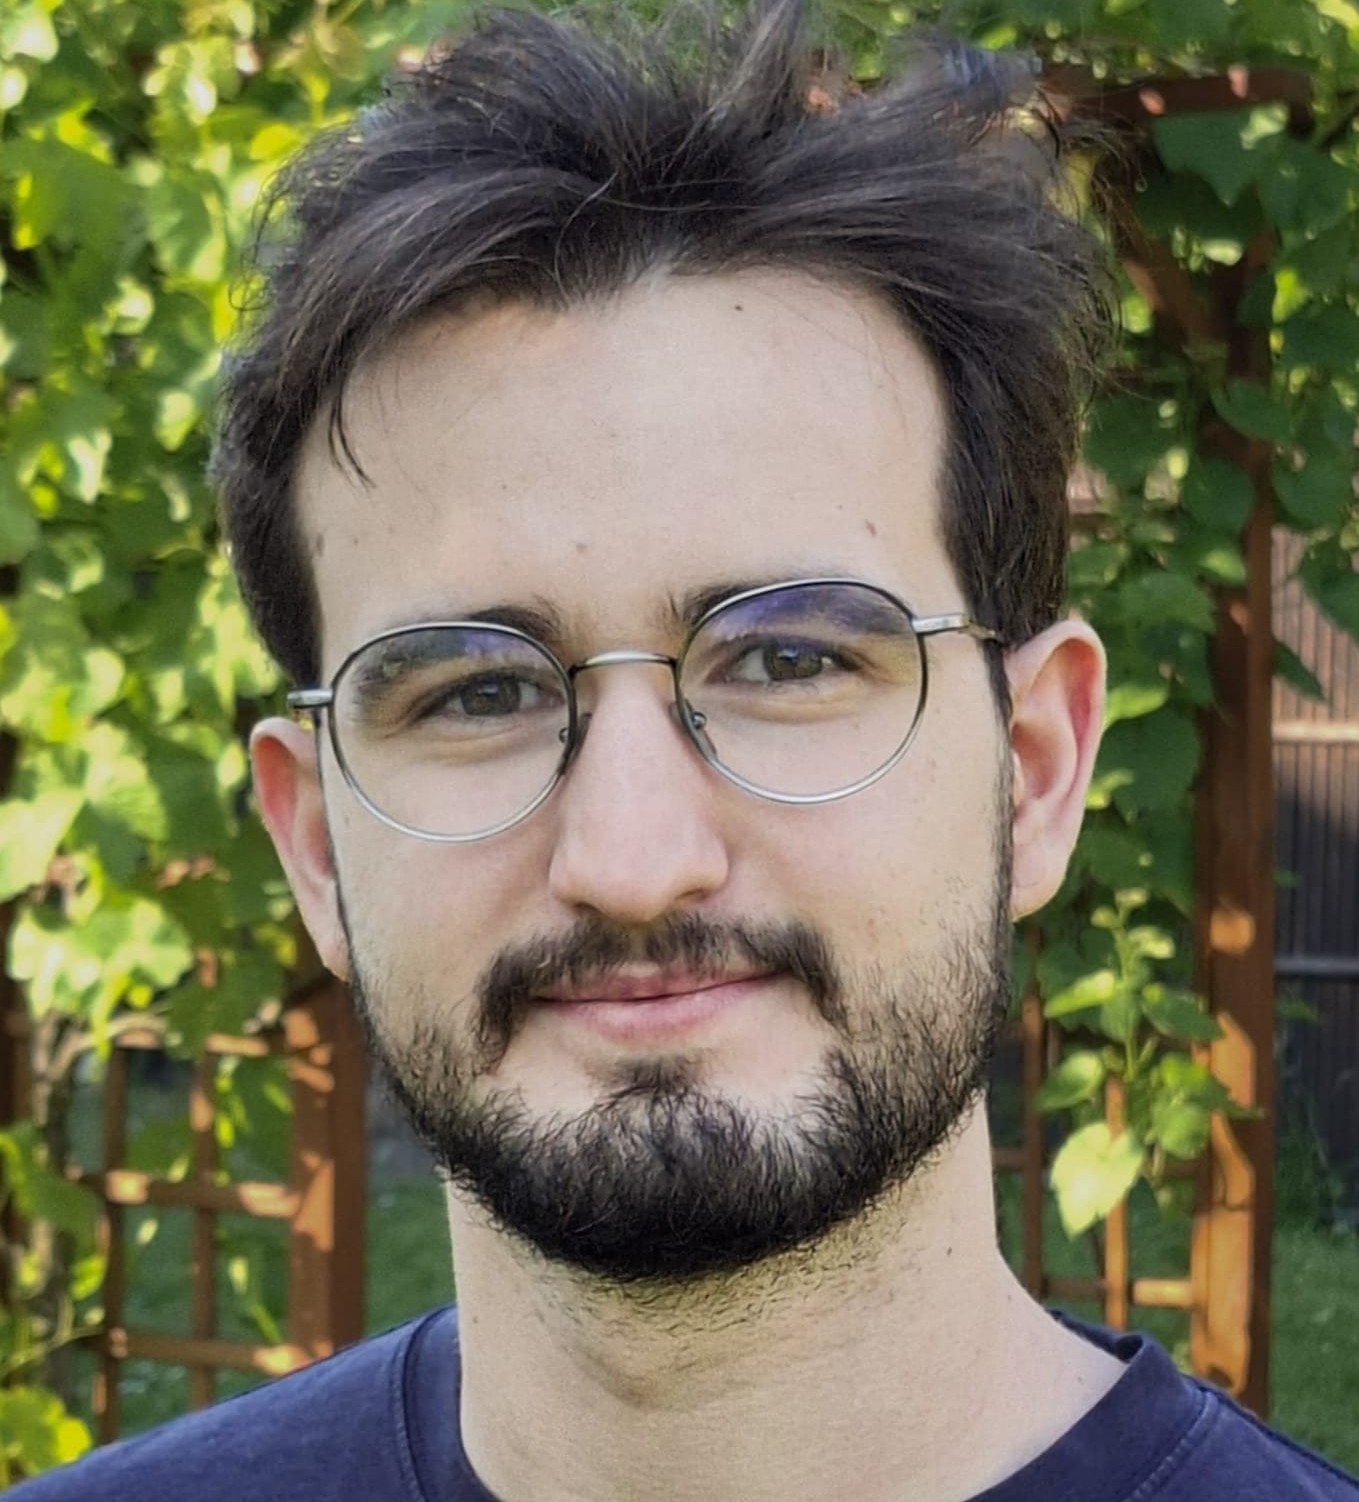
\includegraphics[width=\textwidth]{tronche.jpg} % Remplace 'tronche.jpg' par ton image
\end{minipage} \hfill
\begin{minipage}{0.83\textwidth} % Zone de texte (nom, contact, etc.)
    \Huge{Yoann CORGNET} \\[3pt]
    \large{Étudiant ingénieur en Software Engineering} \\
    \large{À la recherche d'un stage de fin d'études de 6 mois (mai - décembre 2027)} \\
    \large{Postes visés : Ingénieur Logiciel ou Ingénieur DevOps} \\[7.5pt]
    \href{https://www.linkedin.com/in/yoann-corgnet/}{\raisebox{-0.05\height}\faLinkedin\ LinkedIn} \ $|$ \
    \href{https://github.com/Yoann-CORGNET}{\raisebox{-0.05\height}\faGithub\ GitHub} \ $|$ \
    \href{mailto:yoann.corgnet.04@gmail.com}{\raisebox{-0.05\height}\faEnvelope \ yoann.corgnet.04@gmail.com} \ $|$ \
    \href{tel:+33768229430}{\raisebox{-0.05\height}\faMobile \ +33.7.68.22.94.30}
\end{minipage}


%----------------------------------------------------------------------------------------
%	APROPOS
%----------------------------------------------------------------------------------------

%Interests/ Keywords/ Summary
\section{À Propos}
Je suis étudiant ingénieur (ESIEA, double diplôme CentraleSupélec) ; j'ai été responsable technique d'un SaaS \mbox{en production.} Je recherche une mission ou un stage de fin d'études en logiciel : architecture, gouvernance, microservices, systèmes distribués, cloud, DevOps.


%----------------------------------------------------------------------------------------
%	SKILLS
%----------------------------------------------------------------------------------------
\section{Compétences}
\begin{tabularx}{\linewidth}{@{}l X@{}}
Langages  &  \normalsize{JavaScript, TypeScript, Java, Python, C}\\
Frameworks  &  \normalsize{Next.js, Vue.js, Java Spring, Django}\\
DevOps \& Cloud  &  \normalsize{Git, GitHub Actions, CI/CD, Google Cloud}\\
Langues  &  \normalsize{Français (natif), Anglais (TOEIC 970: C1)}\\
\end{tabularx}

%----------------------------------------------------------------------------------------
% EXPERIENCE SECTIONS
%----------------------------------------------------------------------------------------

\section{Experiences Professionelles}

\begin{joblong}{NerionSoft - Développeur Full-Stack}{Sep. 2025 - Auj.}
    \item Responsable technique d’Hestia, moteur de réservation SaaS pour hôtels indépendants
    \item TypeScript, Next.js, PostgreSQL ; architecture hexagonale ; CI/CD GitHub Actions, preview Neon + Vercel
    \item Intégration du PMS Apaleo (OAuth2, webhooks), paiement Apaleo Pay ; application certifiée Apaleo Store
\end{joblong}

%\begin{jobshort}{Sumitomo Electric Wiring Systems Europe - Stage ouvrier}{juill. 2023}
%Filiale du groupe japonais Sumitomo, spécialisée dans le câblage automobile. \\
%Stage d'un mois au pôle IT : rédaction d’un cahier des charges pour un logiciel interne de gestion des notes de frais (analyse des besoins, étude des contraintes légales, conception fonctionnelle, spécifications).
%\end{jobshort}

%Projects
\section{Projets}

\begin{joblong}{Undrive - Projet 4A}{sept. 2025 - févr. 2026}
    \item Application mobile de gamification visant à encourager l’usage des transports en commun par un système de récompenses
    \item Conception de l'infrastructure CI/CD avec Terraform sur GCP, déploiement Cloud Run et gestion des workflows GitHub.
    \item Développement de l'API backend en Django, intégration des microservices Python et base de données PostgreSQL + PostGIS.
\end{joblong}

\begin{joblong}{StockElec - Médaille d'argent (Projet de 2e année)}{2023 - 2024}
    \item Application web de gestion de stock pour le laboratoire d’électronique de l’ESIEA
    \item Développement en méthode agile, avec recueil du besoin client
    \item Frontend : Quasar (Vue.js), Tailwind CSS, tableau analytique interactif
    \item Backend : API RESTful en Java Spring, base de données MySQL, le tout conteneurisé via Docker
\end{joblong}

%----------------------------------------------------------------------------------------
%	EDUCATION
%----------------------------------------------------------------------------------------

\section{Formation}
\begin{joblogo}{0.95cm}{logo-centralesupelec.png}{Double Diplôme CentraleSupélec - Mention Sciences du logiciel}{2026 - 2027}
    \item Génie logiciel : programmation avancée (C++), test, analyse statique, intégration continue, méthodes agiles
    \item Systèmes : systèmes d'exploitation, systèmes concurrents et répartis, algorithmes et modèles distribués
    \item Fondements : algorithmique avancée, logique et systèmes déductifs, sémantique et traitement des langages
\end{joblogo}

\begin{joblogo}{0.55cm}{logo-esiea.pdf}{Diplôme d’Ingenieur ESIEA - Majeure Software Engineering}{Obtention prévue en 2027}
    \item Développement système (C), mobile (Flutter) et Full-Stack (Vue.js, Spring) : SOLID, conception applicative, architecture
    \item Administration Systèmes : Virtualisation, conteneurisation
    \item Data Science \& IA : SQL/NoSQL, analyse de données, Machine Learning, IA
\end{joblogo}

\begin{joblogo}{0.45cm}{logo-uqac.pdf}{Double Diplôme UQAC - Bac+3 en informatique}{2024 - 2025}
    \item Cybersécurité : détection de vulnérabilités (réseau/web), graphes d’attaque (Nmap, Nessus), forensic
    \item Big Data et IA : régression linéaire multivariée, arbres de décision, clustering, réseaux de neurones (MLP, CNN)
\end{joblogo}

%----------------------------------------------------------------------------------------
%	LOISIR / ASSOCIATIF
%----------------------------------------------------------------------------------------

%\section{Associatif et Loisirs}
%\begin{itemize}
%    \item \textbf{Membre actif du BDE}: pôles restauration (budgétisation, préparation, gestion de la caisse) et pôles communication (visuel Canva, rédaction).
%    \item \textbf{Sports et activités}: Escalade, voyages en itinérance (vélo, marche).
%\end{itemize}

\end{document}
